\fancyhead[LO]{{\scriptsize {\FA \ }我们最幸福 {\FA } 买来的老婆}}%奇數頁眉的左邊
\fancyhead[RO]{{\tiny{\textcolor{Gray}{\FA \ }}}\thepage}
\fancyhead[LE]{{\tiny{\textcolor{Gray}{\FA \ }}}\thepage}
\fancyhead[RE]{{\scriptsize {\FA \ }我们最幸福 {\FA } 买来的老婆}}%偶數頁眉的右邊
\fancyfoot[LE,RO]{}
\fancyfoot[LO,CE]{}
\fancyfoot[CO,RE]{}
\chapter*{16 {\FA } 买来的老婆}
\addcontentsline{toc}{chapter}{\hspace{5mm}16 \textbf{>}\ \ 买来的老婆}
\vspace{5mm}
\begin{flushright}
	\textcolor{PinYinColor}{\EN \huge{The\\
	Bartered Bride\\
	\ \\}}
\end{flushright}

\begin{figure}[!htbp]
\centering
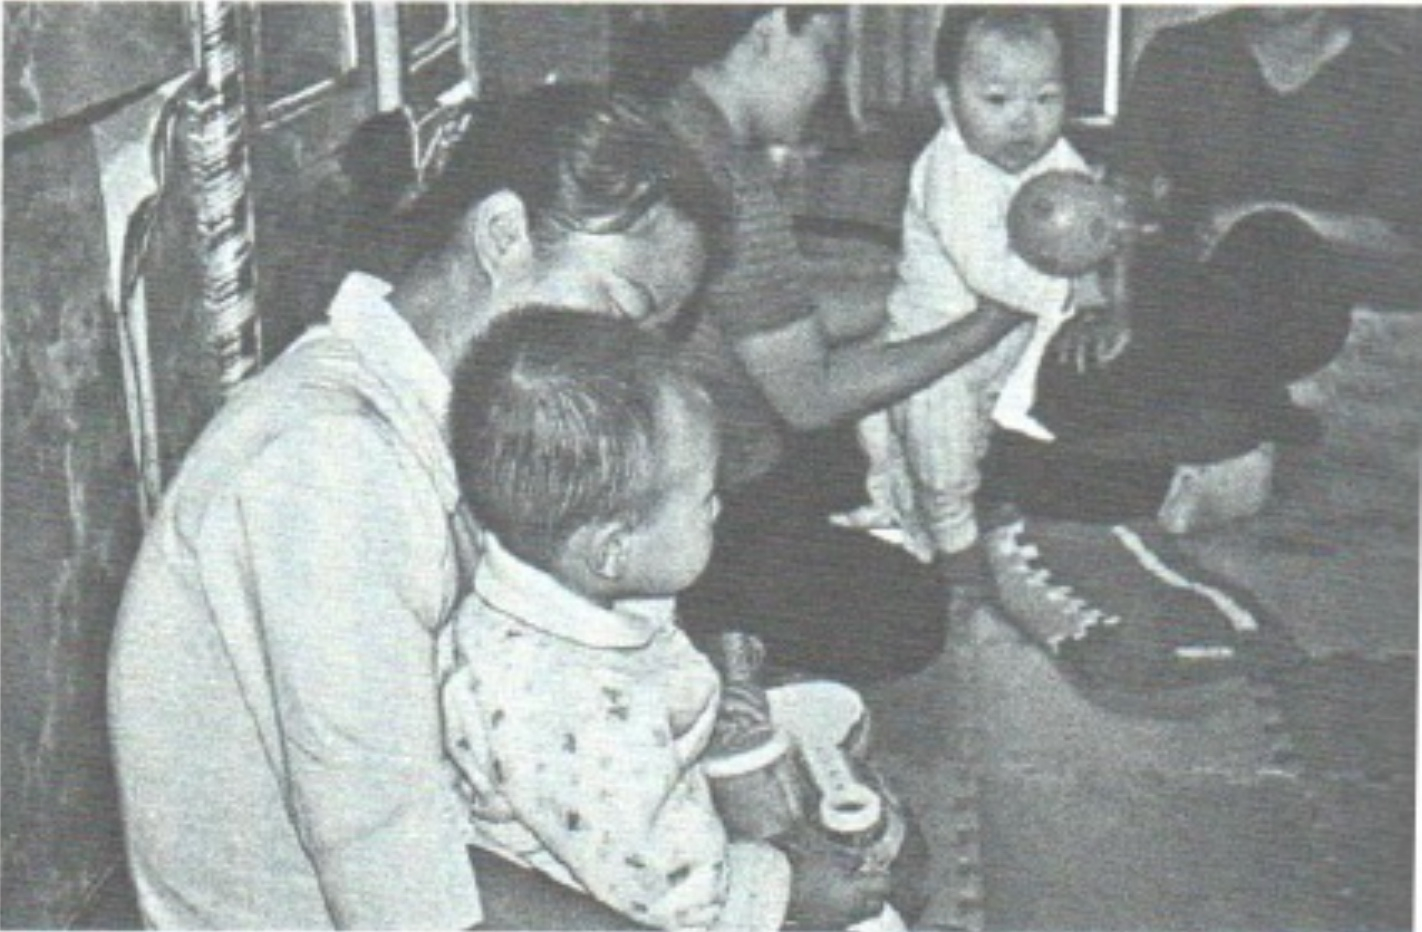
\includegraphics[width=6cm]{./Chapters/Images/16.jpg}
\caption*{2003年中国图门男人的北朝鲜妻子}
\end{figure}

\ifnum\theparacolNo=2
	\begin{multicols}{\theparacolNo}
\fi
一旦有机会,玉熙就会逃离北朝鲜,没人会对此感到吃惊。还是学生的时候,宋女士的这个大女儿就对全国上下对金日成的崇拜敬而远之。从学校一回到家,玉熙就会把少先队的红领巾扯掉。对1994年金日成的死,她也不会刻意假装去哭。\\

过了几年,当全家都在挨饿,她也变得愈加愤怒。她咒骂政府对管理国家经济的无能,咒骂政府让她弟弟和父亲饿死。北朝鲜电视台反复播放一首名为《同志们的行军》的歌曲\footnote{“我们生活在一个社会主义国家,这里衣食无忧。让我们挺起胸膛,骄傲的放眼世界。”}同时屏幕上播放着国旗飘扬的镜头,玉熙认为这简直是愚蠢至极。\\

“不用担心?”她边哼着边把电视给关掉。\\

但是实际上促使玉熙做出叛逃决定的最初动机,不仅仅是要逃离这个系统,也是要逃离她的婚姻。\\

这个婚姻从一开始就被证明是过于草率。玉熙和永洙像其它的夫妻一样,总是为性,为钱争吵不休,后来当日子艰难的时候,他们又为吃的,为政治而争吵。永洙总是能赢。如果争论不是朝他的方向发展,他就会给玉熙个大嘴巴子,把玉熙扇的天旋地转,以此作为总结陈词。\\

尽管酗酒,托家里的福,永洙还是保住了列车员的工作和住的公寓。在铁路系统,列车员可是趋之若鹜的肥缺。当他跑边境的线路时,永洙可以私带货物卖往中国,赚取额外收入。他以5朝元每公斤的价格收购工人从闲置工厂里偷出来的铜线及废金属,再以25元的价格卖掉。起先,玉熙对此很吃惊。因为即使入不了党,她的丈夫以前总喜欢幻想自己是个党干部,喜欢对妻子发表些即兴的、关于邪恶的利己主义和资本主义的长篇大论。他会严厉斥责她对金日成的口出不敬。现在,他却来了个180度的大转弯。\\

“按党的要求做的人是傻瓜。现在只有钱才是王道。”他告诉她。\\

永洙的废金属买卖让他成了困难时期手头较宽裕的人。每次从边境回来,他都能带回家几袋米、几瓶酱油;一时间,他们还在家堆了不少玉米。每次当玉熙提议拿些吃的给她饿肚子的父母时,这都会让他暴怒。\\

“在这个时候,你怎么想着把我们的食物送人?”他大喊大叫道。\\

永洙不信玉熙不会帮衬家里,所以每次他只在家留下刚刚够用的最少量的钱、粮,即使工作使得他回家的时间经常是有几天的来去,而且现在的火车时刻根本无法预计。在1998年,他曾经使得玉熙和他们的儿女,一个8岁、一个6岁,1个星期没有任何吃的。在6月5日,北朝鲜的儿童节\footnote{这里应该有误,社会主义国家都将6月1日作为国际儿童节。──译者},他们的儿子应该参加学校组织的运动比赛。孩子们被告知要自带午餐,但是家里什么吃的都没有。玉熙满城的跑,想从亲戚那里借点粮食,但是没人能有太多的余粮。最后,她在市场找到正在卖饼干的姐姐,抓了些饼干给她。她赶紧跑去学校,在午餐时间,发现儿子站在操场上等着,眼睛里噙满泪水。\\

“对不起,宝贝。”她告诉他,递给他一小袋饼干。\\

永洙,这个曾经的音乐家,有着让女人着迷的、动听的歌喉及优雅的举止。现在,口袋里有了几个钱,就同一帮狐朋狗友,在外面找女人,喝酒到深夜。一天晚上,玉熙和孩子们已经睡着一会儿了,这时候,她听见永洙醉醺醺的闯进门,然后是一个女人的阵阵笑声。玉熙不知道她是永洙的女友还是妓女,但是她不想起来弄清楚。\\

这件事情后,玉熙开始认真的谋划她的逃亡。她可以选择先离婚,但是这样就意味着要失去所有东西。虽然劳动党口口声声要把传统封建社会中地位地下的妇女解放出来,但是北朝鲜的社会体系仍然对妇女不利。如果离婚,男人会留有住房和孩子──而不论是不是因为男方的家暴或出轨。而且由于玉熙的家庭成分不好,加之父亲去世,也没有人为她出头,离婚对她就尤为不利。玉熙心里打算最好能去中国,看自己能不能在那里赚些钱。如果能赚到足够多的钱,自己买个公寓,她可能能获得些筹码,迫使永洙将孩子的监护权给她。\\

一天晚上,永洙喝醉了回家,而且脾气特别不好。他打了玉熙,把她推到在地,然后狠命的踢了一脚,以至于玉熙仿佛听见自己肋骨断裂的声音。突然有人敲门──是个过路人来问路,由于住在火车站附近,所以常有人来问路。当她丈夫答应的时候,玉熙从地板爬起来,退到了厨房。打开后门,只穿着睡衣她就沿着台阶走下去了。\\

火车站的时钟显示当时的时间是晚上10点。时值8月底,晚上气温还比较宜人。当离家足够远,确信丈夫没有跟来后,她在外面站住了,仔细考虑下一步该怎么做。通常冲突之后,她会跑回娘家,母亲会用热毛巾帮她敷一敷豁着的嘴唇和青着的眼圈。第二天早上,当永洙清醒过来,他会哭着道歉,求玉熙跟自己回去,而她也总是会这样做。10年了,他们就一直这样生活着。如果她想改变,现在就是时候了。\\

玉熙不敢去清津火车站,那里有很多丈夫的同事可能会认出她来。因而,在暖风吹拂下,她整夜都沿着铁道向北走,先是出了城,然后来到了位于郊区的第一个火车站,寿城。现在无家可归的人非常多,没人会注意一个只穿着睡衣的女人。\\

她在这个火车站待了两天。她的肋骨因为那一脚现在还一阵阵抽搐的痛。饥饿和脱水也让她隐隐觉得头疼。她也因为头晕目眩而无法站立。她看见一群人聚在火车站,人们看上去都很兴奋。一趟火车马上要开车了,前往边境城市茂山。她鼓起全身的力气,努力的冲入想从门和窗户爬上车的人群。人们抢着座位,之后填满走道,站进厕所,最后连车厢间的过道都挤满了人。还有些人挂在窗户上,附在车厢底。车厢挤满了人,列车员根本无法通过去检查车票和旅行许可。在走了一天之后,玉熙来到了茂山。现在的玉熙一无所有,没有身份文件,没有钱,没有吃的,没有衣服。\\

她现在有的只是一个32岁女人还算健康的身体。玉熙从来都不算非常漂亮。她母亲过去常常把她定位为最聪明的女儿,而她第二个妹妹每个人都说她长得像电影明星,但是玉熙在饥荒中的境况比其它人好。和母亲一样的娇小丰满,她还有着让人会误认为肥胖的体形。她的小鼻子,让她看上去很年轻,牙齿又白又整齐。然而即使看上去很显年轻,但是她还是太老了做不了妓女,而且这也不在她考虑的范围之内。然而,对北朝鲜妇女来说,还有另外一种方式可以把自己卖了,而且这种方式还更让人心甘情愿。\\

就在图们江对面,那里的玉米地延绵几公里。那里的村子里有足够的吃的,但是他们缺女人。在想生儿子的传统,和控制家庭人口的政策之下,导致新生儿中性别比例失调,每13个男性,对应10个女性。在十几岁的时候,很多年轻女孩都涌向城市,在不断膨胀的工厂里找到工作,那里她们的薪水比种地好多了。乡村里的光棍,特别是35岁以上的没有钱或者没什么个人魅力的就很难找到老婆。他们转向那些婚托求助,而婚托一般对他们的服务只收取300美元,当然如果介绍的妇女既漂亮又年轻,他们也会多收一点。但是漂亮和年轻不是必要的前提条件;身体健康的60岁老妇也有人要,可以帮一些更年老的鳏夫煮饭,操持家务。北朝鲜妇女对中国人来说还有那么一些的神秘。尽管因为饥荒,身体、面容大不如前,但是北朝鲜妇女仍被认为是亚洲女性中最漂亮的之一。南韩男性经常谈论这:北女(Buk nyeo)、南男(Nam nam),据称是最理想的基因组合。中国男人发现北朝鲜的女人比中国的媳妇的更谦卑和顺从。\\

玉熙对中国人买卖婚姻的市场很了解。当清津有妇女神秘消失了,人们就会咬耳朵,“那个贱妇可能把自己卖到中国去了。”\\

茂山的火车站就是这些买卖起始的源头。一个妇女只需要在那里单独的逛逛,就会有出价自动靠上来。那个给玉熙拉生意的男人后来才知道是她丈夫的一个老朋友。他给玉熙提的条件是:会有一个向导带她过河去中国。她会得到衣服、内衣、吃的和一的临时的住地直到配对成功。婚托会帮她找个体面的人家,她去给人家做老婆,其实各方都清楚,这种婚姻不会被中国法律所承认。作为回报,她同意和为她选的男人待在一起,且她一分钱也拿不到。\\

玉熙同意了这些条件,并提了一个要求。她坚持这个男人不说朝鲜语。大多数的北朝鲜妇女都倾向于同一个朝鲜族的男人生活,这样他们交流起来没有障碍,但是玉熙不是。\\

“不要朝鲜族。”她告诉婚托。“我想生活在一个没人认识我的全新的世界里。”\\

这个人帮玉熙选了一个三十过半的农民。他非常矮,大概150公分,和她一般高。他看上去呆呆的,以至于玉熙怀疑他是不是有点轻度的弱智,而且他非常害羞,都不敢正视玉熙的眼睛。毫无疑问,他肯定没结过婚,她想。他们在边境靠中国一侧的一家小饭店里见面。同她一道到中国的,另外一个北朝鲜妇女则被卖给了一个个子高些的,也更有生气的男人;他同陪同的其它人有说有笑的。玉熙感到有点嫉妒,但是她提醒自己这是她的选择──她想要一个她不可能爱上的男人。\\

数以万计的北朝鲜妇女就这样被卖给了中国男人。根据一些估计,居住于中国的大约10万名北朝鲜难民中,有3/4是妇女,其中一半是以这样的方式同中国男人在一起。关于北朝鲜妇女被殴打、被强奸成串被关押或者像奴隶一样被奴役的遭遇,简直就是一部血泪史,罄竹难书。然而,玉熙却是非常幸运。玉熙的这个男人名字叫明远(Min-yuan),他没有一点自己丈夫的那种魅力,但是他却非常体贴,使得他看上去对这个世界来说太过于无知。第一次和她上床的时候,他抱着她,用盆子打来热水给她洗脚。他给她做好吃的,不让她下厨。他的父母也是一样的疼爱她。\\

玉熙同这个男人差不多生活了两年多。她也学了足够多的中文,所以他们之间可以交流。她仔细阅读一本孩子的地理书,所以她可以自学中文。期间她住在山东,那是离她跨境地点西南1000公里之外的地方;是位于青岛以西的一个富产棉花和小麦的农业大省\footnote{这里作者有误,青岛是山东的一个市。──译者}。她记住进城的公交路线。这些日子里,她一直在策划出逃。\\

她怀了两次孕,但是都打掉了。虽然明远很想要个孩子,她还是说服了他,如果生下来,这个孩子注定命苦。中国政府是不会承认他同北朝鲜妇女的婚姻,所以他们的孩子无法注册成为公民,这样就上不了学。\\

“我在北朝鲜已经有两个孩子了。总有一天我要回去找他们的。”她告诉他。明远很难过的点点头。\\

当她决定要走的时候,明远送她到车站,给了她100元。他哭了。她也希望他能求她留下来,但是他没有。他还是像她第一次见到他时一样的木讷。他只是告诉她,“小心点。”。\\

实际上,玉熙的旅途充满艰险。到2000年,中国人开始对脱北者感到厌倦了。太多了,他们有点担心了,这些脱北者可能会抢走中国人的工作、打破中国东北地区的稳定并引发民族骚乱。人权主义者认为中国政府在道义上和法律上,有责任给这些叛逃者以食物和住所。但是中国坚称这些跨界的人属“经济难民”并不属于中国签署的《联合国难民地位公约》(Convention Relating to the Status of Refugees)中所需提供保护的难民。中国人还指出之前同北朝鲜国家安全部于1986年签署的秘密协议,该协议要求双方合作打击非法越境者。\\

中国人会定期展开抓捕脱北者的专项行动。他们在靠近边境的地区设置检查站,随机检查身份证。在中国几个月后,北朝鲜人一般都会胖起来,也买了新衣服;因此很难将他们同中国人区别开来。所以中国人允许北朝鲜警察入境找出他们的国人。还有脱北者自身被发展成为间谍,去筛查其它脱北者的藏身之所。中国政府也悬赏40美元给举报有北朝鲜女人同中国男人生活的告密者。这些妇女会从家里、从她们事实的丈夫、从孩子身边被带走。男人会被罚款,但是可以留下他们的孩子。在2000年3月的一轮这样的行动中,就有至少8000名妇女被逮捕\footnote{直至2008年,这样针对脱北者的抓捕行动仍在中国持续着。}。\\

玉熙在中国丈夫的村子里很安全,因为那里离北朝鲜的边境足够远,以至于在抓捕范围之外。但是为了赚钱,她要不得不回到边境地区,在那里有很多朝鲜语的使用者,因此机会也更多。她非常渴望赚钱──这是她唯一的机会去买来自己的自立和孩子的监护权。吃好,休息好后,她试图在餐馆或者工厂找份工作,然后也许能自己做点小生意。她坐上向北驶去的客车,不是回她跨境的地方,而是去了丹东,中朝边境最大的城市。\\

丹东是个兴旺的城市。鸭绿江沿岸,新建的办公楼、公寓楼的玻璃幕墙熠熠生辉,林立的塔吊混杂期间。对比于与江对岸北朝鲜的肃杀,丹东的繁荣就更显得震撼。然而丹东对玉熙来说,很快就被证明不是个明智的选择。连接平壤与北京的主要铁路穿过这个城市,很多官方贸易也通过跨过两国的中朝友谊桥完成。北朝鲜很多国有商社在丹东都有办公室。这个城市遍布着便衣特工。\\

玉熙是在2001年的1月被捕的,并被递解过江,遣送至新义州的警察局。经过2年在中国的生活后,玉熙被自己国家的状况震惊了。数九寒冬,警察局里没有暖气。警察和囚犯们一起都被冻得瑟瑟发抖。一个警察在一个木片上写下了对她的指控,他们连纸都没有。然而,她的时机很巧。为庆祝金正日的生日,有个大赦即将来到;数以千计的罪行较轻的罪犯将被释放。在被关押了仅仅2周之后,玉熙就被释放了。刚被释放,玉熙马上就又过江去了中国。\\

在被捕前,玉熙在一家砖厂工作过,之后又去了一家餐馆。每天赚那么1块钱、2块钱都是她的财富──这可相当于在清津一个月的工资──但是这在中国算不了什么。这次,玉熙需要找份能赚更多的工作,即使这意味着要冒更大的风险。她决定也做个经纪人,就像那个把她卖给中国农民的那个男人一样。她第一份差事要她潜回北朝鲜,找个被留下来的孩子,并带他跨过图们江和他的家庭团聚。玉熙接下了这单生意。\\

这个孩子据信应该住在茂山,她第一次出逃时的出发地。她对这个城市很熟悉,甚至可以说当地的方言,所以她想她能在哪里转悠几天而不会引起太多的注意,但是她错了。她刚到茂山的第一天,一个警察就把她从人群里提了出来。\\

“嘿,你。”他朝她喊道。经过两年多的中国生活,玉熙现在又白又胖。她习惯了用带有香味的香波和香皂。这使得她看上去和所有的人都不一样。此外,她还带了个在中国买的,可以收听到南韩节目的半导体收音机。警察没收了她的收音机\footnote{警察让她告诉他们南韩广播节目的频道,然后又要走了她的耳机。}然后再把她移交给了保卫部。\\

玉熙被投入一个收容间,里面装有100多个被逮捕的人。他们都被告知跪着,不许动。警卫在一排排之间来回巡视,如果有人想动动跪麻的腿,马上就会遭致他们的殴打。在也被打了一次之后,玉熙只能用眼睛四处瞟瞟。在仔细看了看同被关押着的人后,她马上就能说出谁在中国待过。那些皮肤白皙,穿戴较好的,看上去气色不错的就是和她一样的。其它的人,憔悴、面黄肌瘦,通常都光着脚;他们可能是还没跨境就被逮着了。\\

玉熙想还好,这两种人都混在了一起。她最好的生存机会就是当局不知道她是个经纪人。她也希望那个没收她收音机的警察能自己留着那个收音机而不要上报。对叛逃者的惩罚不一而论,要看阶级成分,和叛逃者在中国做了什么。如果仅仅是过界找吃的,那么惩罚就会比在中国生活、工作来的轻。那些拐卖妇女、买卖DVD影碟、同南韩人见面或者去过在中国的教堂的人,就会被控以“背叛祖国”,一般都被处以极刑或者关进古拉格。\\

最后,警卫们按照籍贯,把收容室内的人们进行分类。当分好之后,玉熙发现很多人都是来自清津。警卫们没有手铐,所以他们3个人一组用塑料鞋带把他们的大拇指绑在一起。这些带子绑的非常紧,以至于血液无法流通,整个大拇指都淤青了。囚犯们之后被押送上了一列专列,他们三个人被塞入原本两个人坐的位置。玉熙看到过道对面一个人艰难的在口袋里翻找着什么东西。那人设法藏了个打火机。他用打火机烧断了绑着的塑料带,然后三个人在警卫发现之前都翻窗逃掉了。女人们不敢动,除非有一个人不得不去上厕所;如果那样,那么三个人就要大拇指连在一起的一起去。\\

当列车发出刺耳的刹车声时,玉熙意识到她到清津火车站了。时间是2001年的9月,差不多离她穿着睡衣跑出来的那天有3年了。现在她灰溜溜的回来了,被绑着大拇指,像个被用锁链锁住的囚犯一样,回来了。\\

“Baka,baka。”──低头,低头,当囚犯们爬下车的时候,警卫们大声呵斥着。\\

玉熙更情愿低着头。如果被丈夫或者他的同事看见怎么办?他们列队穿过火车站候车室,走过她妈妈卖饼干的广场,然后正好从她家窗户下经过。在过去,她自己经常会透过那扇窗户扫视那些成群的囚犯,看看有没有自己认识的人。\\

然后他们被领着沿着清津的主干道走下去,穿过一大群好奇看热闹的人,然后再跨过两座桥,走过工业区和沼泽一样的洼地,那里是清津唯一可以有稻田的地方。之后再转向大海的方向,他们来到了一个被混凝土高墙和铁丝网环绕的院子。这个地方就是农浦拘留中心,建于日据时代,用于关押朝鲜的抵抗份子。农浦这两个字就意味着死亡。现在里面关押的满是叛逃未遂的人们。\\

女囚就满满三大间,非常拥挤以至于女人们只能侧过来成排的睡在地板上。那些找不到地方的就只能睡在厕所里了。每隔几天就有更多的犯人到达,通常一次就有上百人。警卫们对新来的都要进行裸体搜身,把明显怀孕的挑出来然后送去强制堕胎,而不论胎儿是不是几乎就要降生了。他们都假设孩子的父亲是中国人。\\

在农浦男女囚犯的比例大概是1:2,这也大致反应了脱北者的一个性别比例。当玉熙和其它女人熟识之后,她很吃惊的发现她们的经历和自己的是多么的类似。很多人都是离开丈夫和孩子,都辩称自己想着能给家里带些钱和吃的回来。玉熙对这些女人感到恶心,当然也对自己感到恶心。她永远不能原谅自己抛弃了她的孩子们。我们都变成了怎样的少廉寡耻的贱女人。饥饿让我们丧尽天良,她想。在里面,她有大把的时间好好反省。长时间的奴役之后紧接着的是漫漫长夜的自我批评和学习。囚犯们食不果腹,动辄挨打。总的看来,其实农浦可能比其它的监狱还要好一些。在周六的下午,女犯允许从院子的井里打些水洗个澡。她们相互帮忙在头发里抓虱子。在待在里面的时间里,她只一次看到个女人被暴打。那次是在气愤之下,这个妇女试图爬上围着院子的一堵墙。其实也就是耍耍泼,而不是真正的意图越狱,而且她也没有机会逃脱,但是警卫把她拉下来,当着其它囚犯的面,拳打脚踢的把她打的神志不清。\\

总的来说,在农浦的女犯给玉熙留下的印象是愤怒多于害怕。当她们被强制要求劳动的时候──制砖、田里除草──她们的脸上永远愤怒的扭曲着。我们一辈子都在听谎言。我们的生活就是一个谎言。整个系统就是个谎言,玉熙认为,而且她也确信其它女人的想法和她一样。\\

这里每一个监狱教官都放弃了再教育。他们仅仅走个形式,麻木的读读劳动党分发的学习材料。每个人看上去都活在谎言里。\\

有一天,当女犯被安排去收割玉米,监狱长跑来在玉米地做了一个即兴演讲。这是常有的事情。他要求她们用金日成思想武装自己,自觉抵御资本主义诱惑,献身祖国。\\

然后他要求大家举手示意:谁发誓再也不跑去中国?女人们一个个都气鼓鼓的蹲在地上。玉熙环顾四周。没有一个女人举手。在一阵令人不安的沉寂之后,监狱长说话了。“好吧,如果你们还想去中国,下次不要被抓住了。”\\

实际上,玉熙已经在谋划好下一步的行动。一天,她被派去给菜地除草,菜地位于高墙之外,有刺铁丝网形成的栅栏之内。玉熙看见一个年长的妇女在附近,在栅栏另外一边放羊。玉熙迅速看看左右,没有警卫在附近。她透过栅栏和这个妇女说话。她想和她做个交易:玉熙把自己的内裤给她,如果她能去找玉熙的妈妈并捎个口信说她在这里的话。内裤在北朝鲜算是稀有之物,而且玉熙的内裤还是新的,刚刚在中国买的。这个妇女同意了。\\

玉熙蹲下来,脱下了内裤。她把内裤揉成一个球,塞了个写着母亲地址的纸条,扔过了栅栏。\\
\ifnum\theparacolNo=2
	\end{multicols}
\fi